\subsection{Architectures}

\begin{frame}{Architectures}
	\begin{block}{Usual building functions}
		\begin{itemize}
			\item 2D Convolution
			\item Non linear function (ReLU)
			\item Batch Normalization
			\item Pooling (mean/max)
			\item Fully connected layer (MLP)
		\end{itemize}		
	\end{block}
	
	\begin{block}{Usual buildings "block"}
		\begin{itemize}
			\item \textit{Features extraction:} Conv + Batch Norm + Relu + Max pooling
			\item \textit{Classification} FC + SoftMax
		\end{itemize}
	\end{block}
\end{frame}

\begin{frame}{Famous nets: Alexnet}

	\begin{figure}
		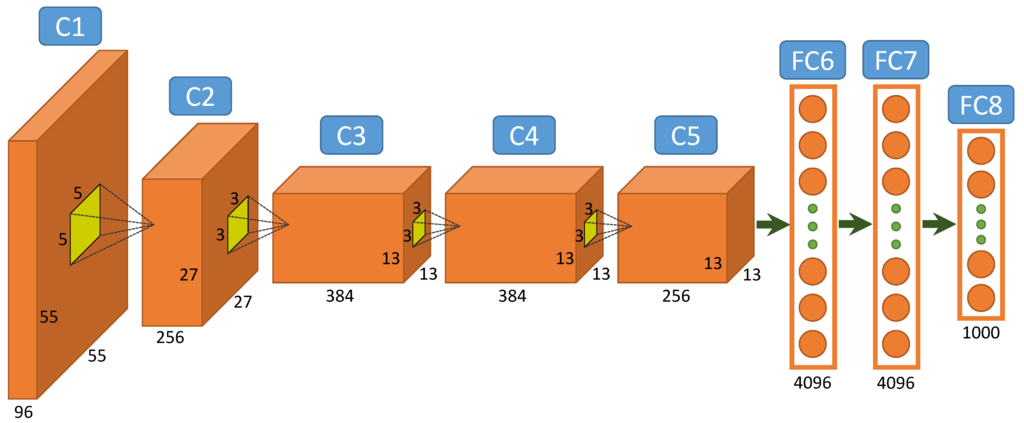
\includegraphics[width=\linewidth]{images/alexnet.png}
		\caption{Alexnet}
	\end{figure}
	
	\cite{ALEXNET}
\end{frame}

\begin{frame}{Famous nets: VGG}

	\begin{figure}
		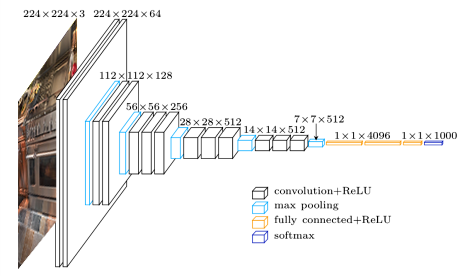
\includegraphics[width=0.5\linewidth]{images/vgg.png}
		\caption{VGG16}
	\end{figure}
	16 vs 5 convolution for Alexnet	
	
	
	\cite{VGG}
\end{frame}

\begin{frame}{Famous nets: GoogLeNet}

	\begin{figure}
		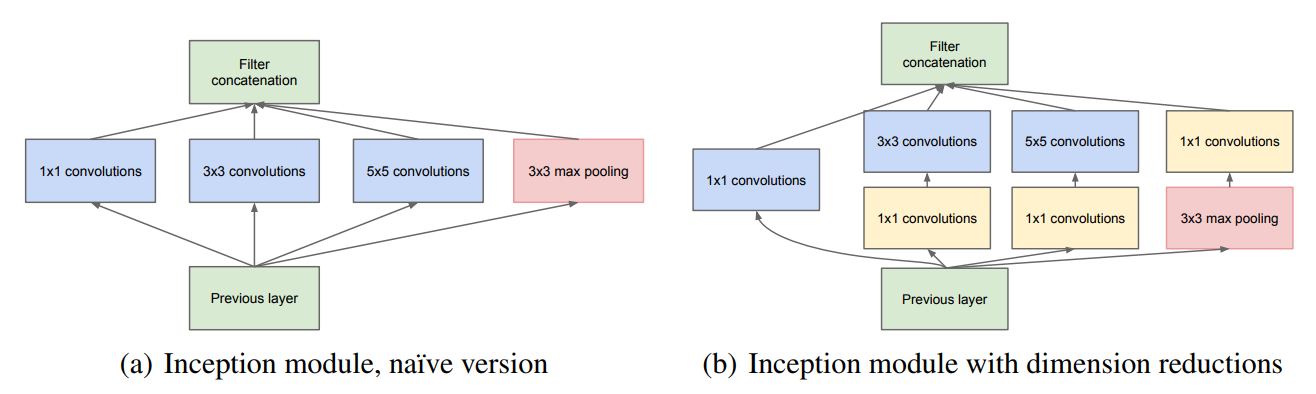
\includegraphics[width=\linewidth]{images/inception.png}
		\caption{New inception module}
	\end{figure}
	Convolution on smaller input = put more convolutions
	
	
	\cite{INCEPTION}
\end{frame}

\begin{frame}{Famous nets: ResNet}

	\begin{figure}
		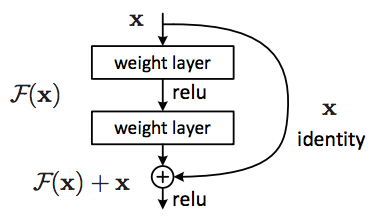
\includegraphics[width=0.5\linewidth]{images/resnet.png}
		\caption{Residual block}
	\end{figure}
	Residual networks easier to optimize = put more convolutions (8xVGG)
	
	
	\cite{RESNET}
\end{frame}

\begin{frame}{Famous nets: DenseNet}

	\begin{figure}
		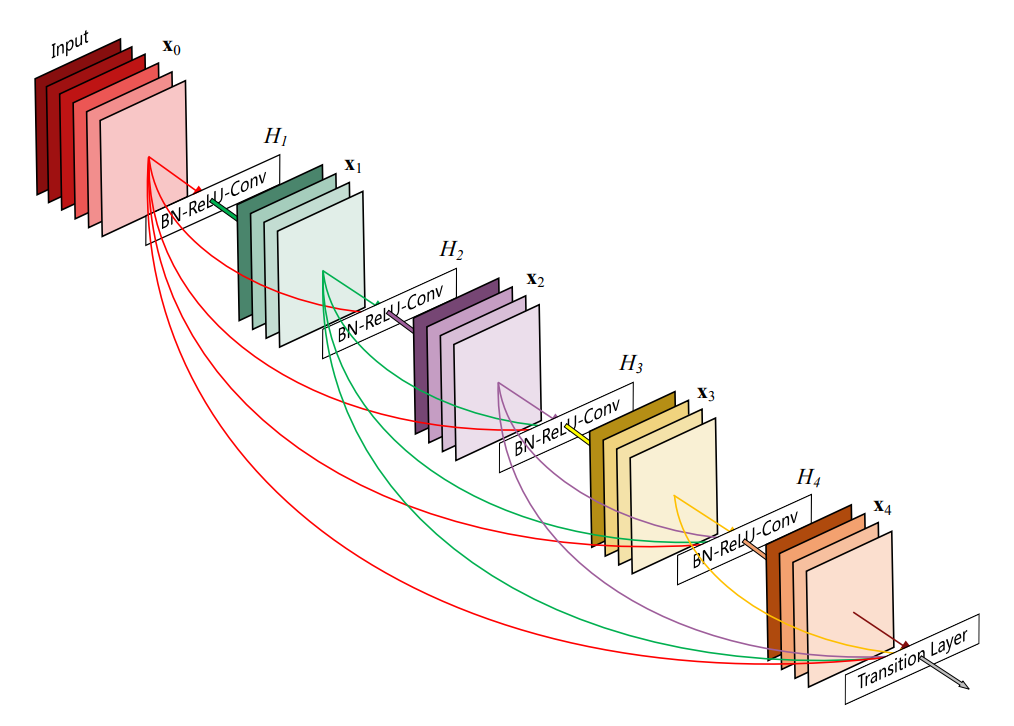
\includegraphics[width=0.5\linewidth]{images/densenet.png}
		\caption{Dense block}
	\end{figure}
	Less parameters for similar results (CVPR2017)
	
	
	\cite{DENSENET}
\end{frame}


\subsection{Recurrent Networks}
\begin{frame}{Temporal informations in DNN}
	\begin{figure}
		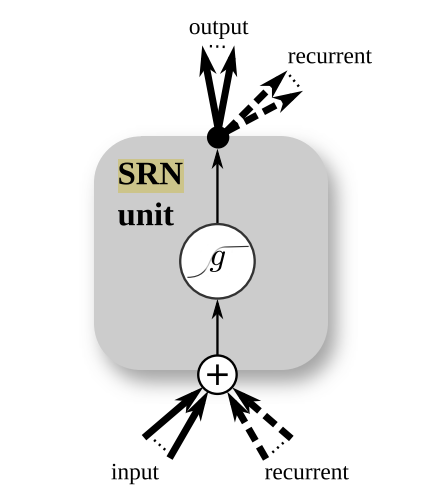
\includegraphics[width=0.2\linewidth]{images/srn.png}
		\caption{Simple Recurrent Network}
	\end{figure}

	Can be applied on sequential data: speech, video, graph...
	
	\begin{block}{More complex RN}
		\begin{itemize}
			\item Long Short-Term Memory (LSTM)
			\item Gated Recurrent Unit (GRU)
		\end{itemize}	
	\end{block}
\end{frame}

\subsection{Applications}
\begin{frame}{CNN Applications}
	In computer vision, deep learning have been first applied for image classification, with:
	\begin{itemize}
		\item CNN for features extraction
		\item MLP for classification
	\end{itemize}
	All the weights (CNN + MLP) are optimized within a common framework \textbf{end-to-end}.

	\hfill
	
	DL are now used in others computer vision applications.
\end{frame}

\begin{frame}{Application: Keypoints detection/description}

	\begin{figure}
		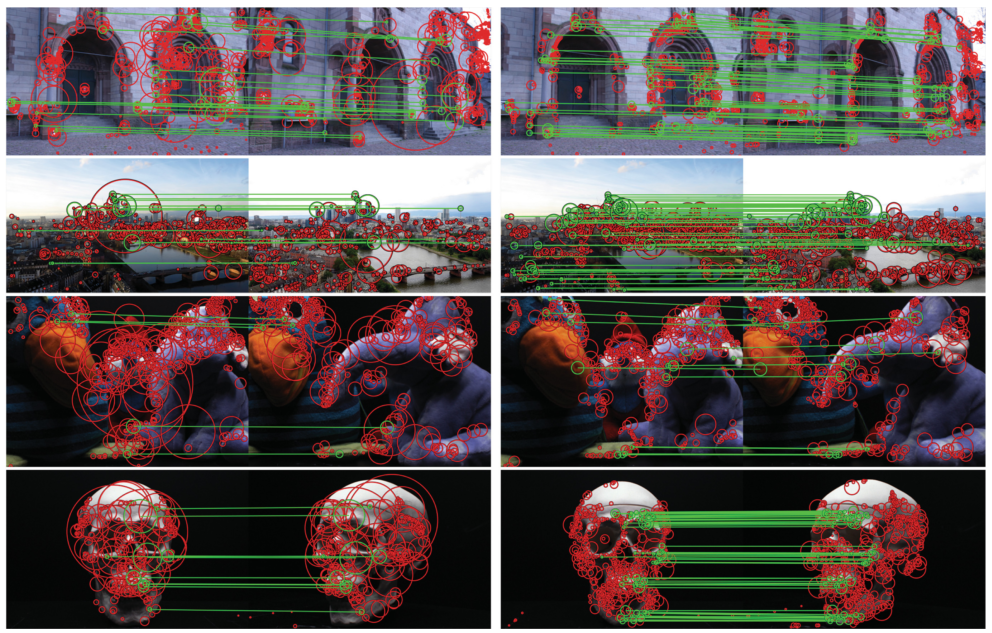
\includegraphics[width=0.8\linewidth]{images/lift.png}
		\caption{SIFT vs LIFT}
	\end{figure}
	
	
	\cite{LIFT}
\end{frame}

\begin{frame}{Application: Region Proposal Network}

	\begin{figure}
		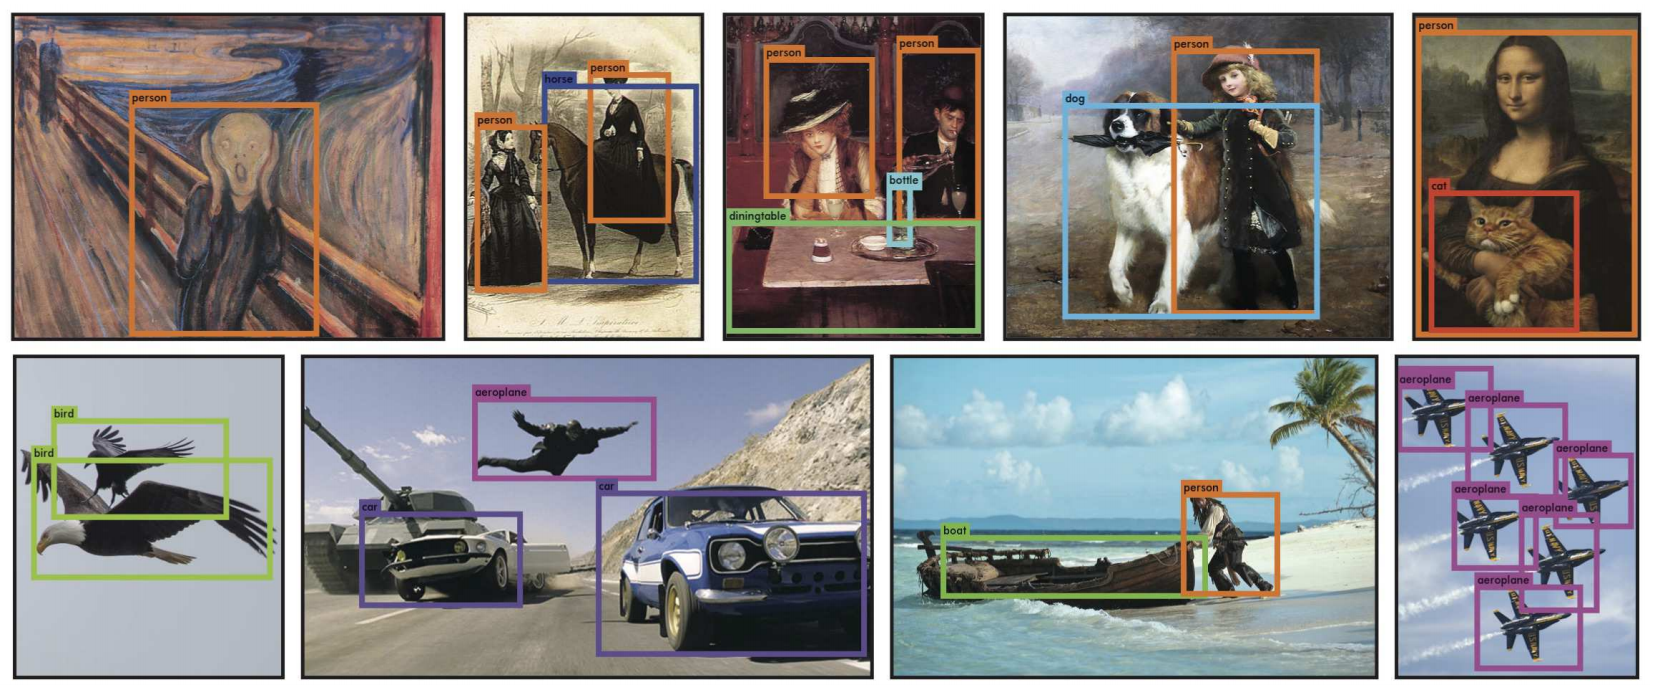
\includegraphics[width=\linewidth]{images/yolo.png}
		\caption{RPN network}
	\end{figure}
	
	Multi-task learning network (Region proposal \& classification)
	Best Paper CVPR2017~\cite{YOLO9000}
	
	\cite{YOLO,FASTRCNN,FASTERRCNN}
\end{frame}

\begin{frame}{Application: Pixel-level Segmentation}

	\begin{figure}
		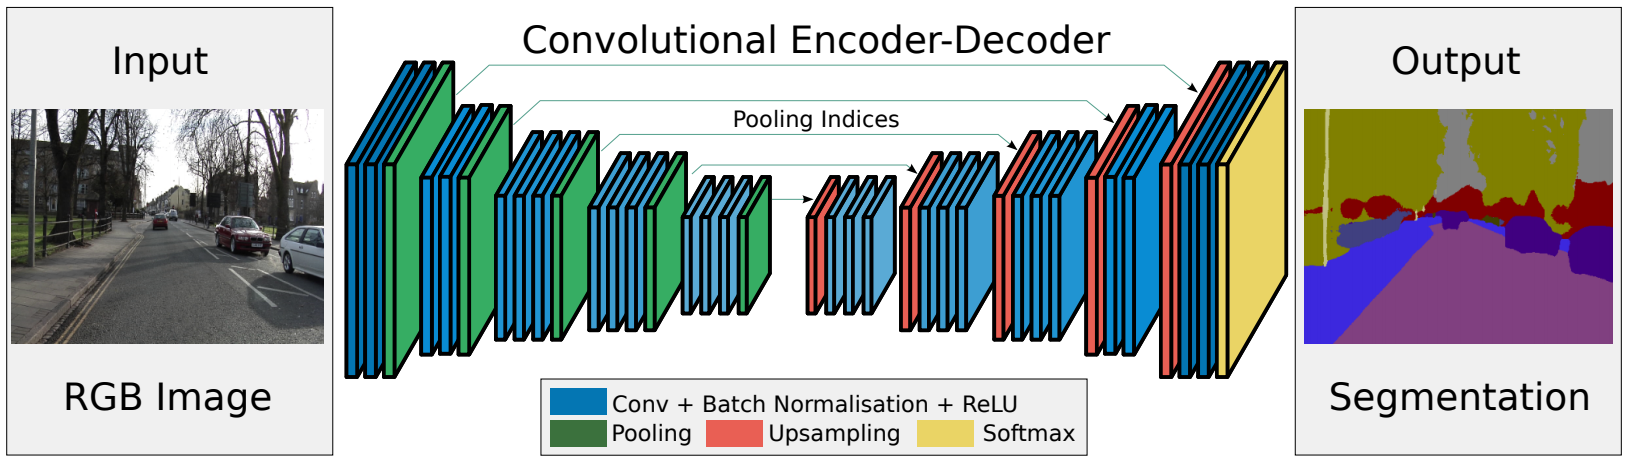
\includegraphics[width=\linewidth]{images/segnet.png}
		\caption{Encoder-Decoder architecture for semantic segmentation}
	\end{figure}
	
	Introducing max-unpooling to obtain an output as wide as the input.
	
	\cite{SEGNET}
\end{frame}

\begin{frame}{Application: Instance segmentation}

	\begin{figure}
		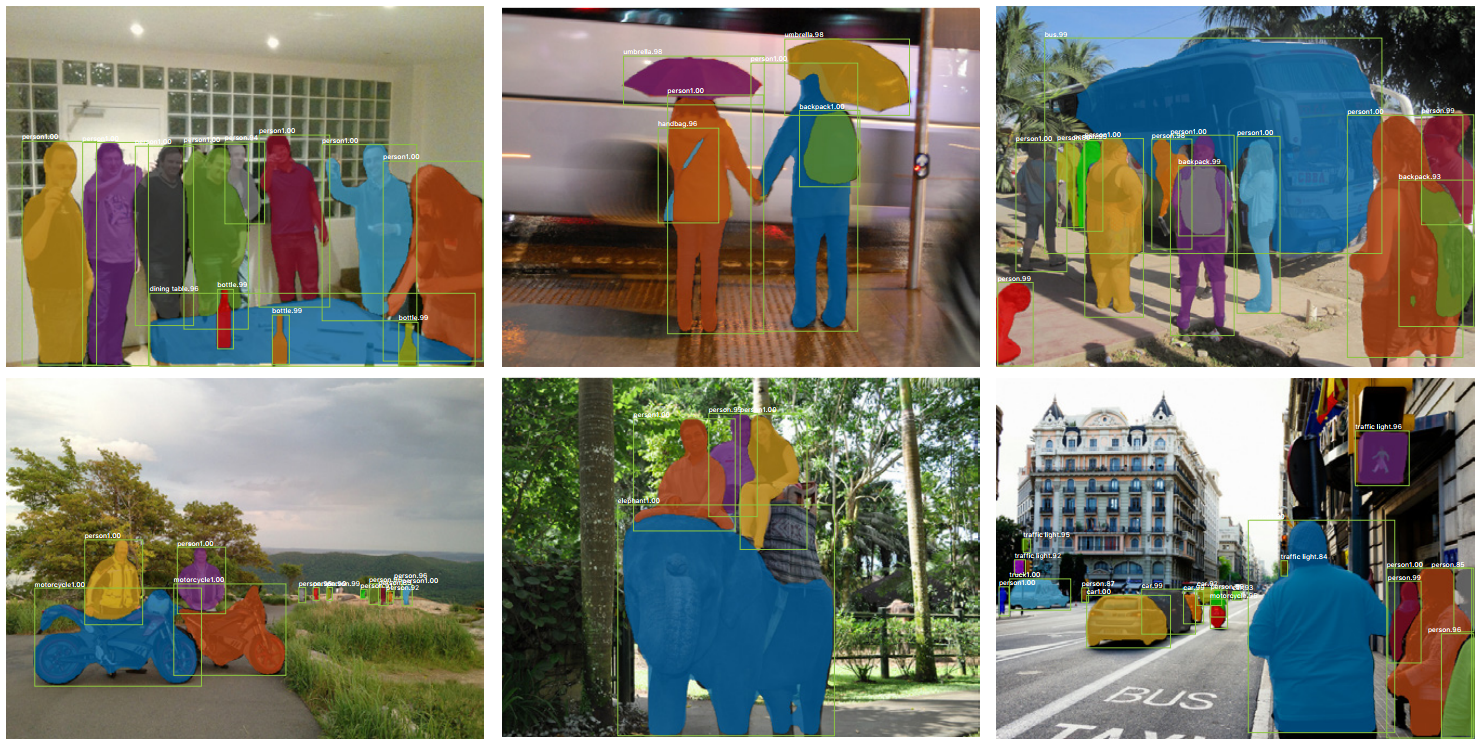
\includegraphics[width=\linewidth]{images/maskrcnn.png}
		\caption{Instance and pixel-level segmentation}
	\end{figure}
	
 	Best Paper ICCV2017~\cite{MASKRCNN}
\end{frame}

\begin{frame}{Application: Depth from stereo}

	\begin{figure}
		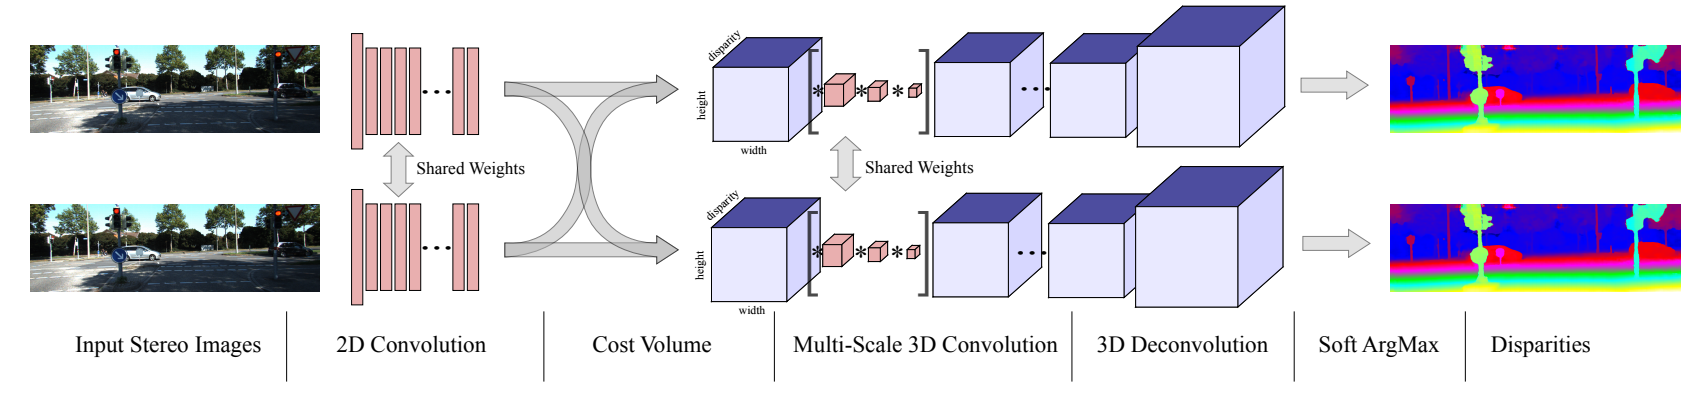
\includegraphics[width=\linewidth]{images/gcnet.png}
		\caption{Disparity inference from stereo pairs}
	\end{figure}
	
	Double-inputs network
	
	\cite{GCNET}
\end{frame}

\begin{frame}{Application: Depth from mono}

	\begin{figure}
		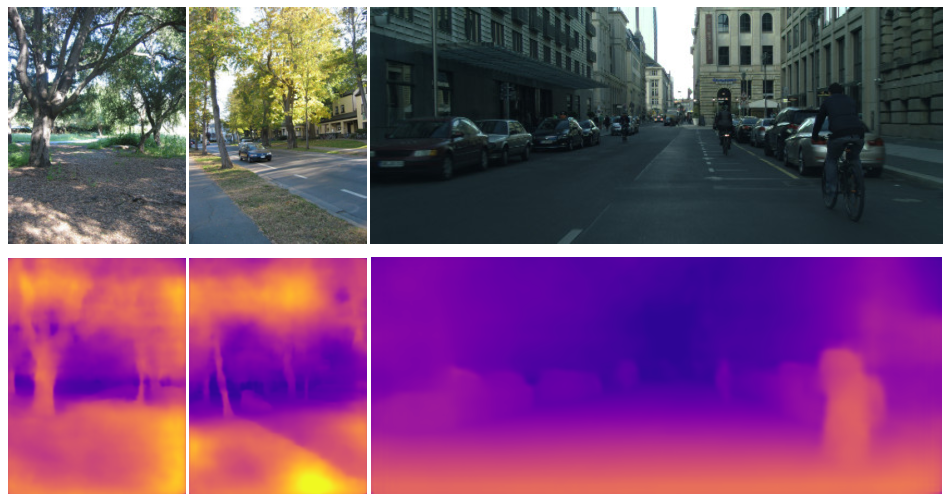
\includegraphics[width=0.8\linewidth]{images/mono2depth.png}
		\caption{Disparity inference from mono image}
	\end{figure}
	
	Used to improve monocular SLAM~\cite{CNNSLAM}
	
	\cite{MONO2DEPTH}
\end{frame}

\begin{frame}{Application: Visual Odometry}

	\begin{figure}
		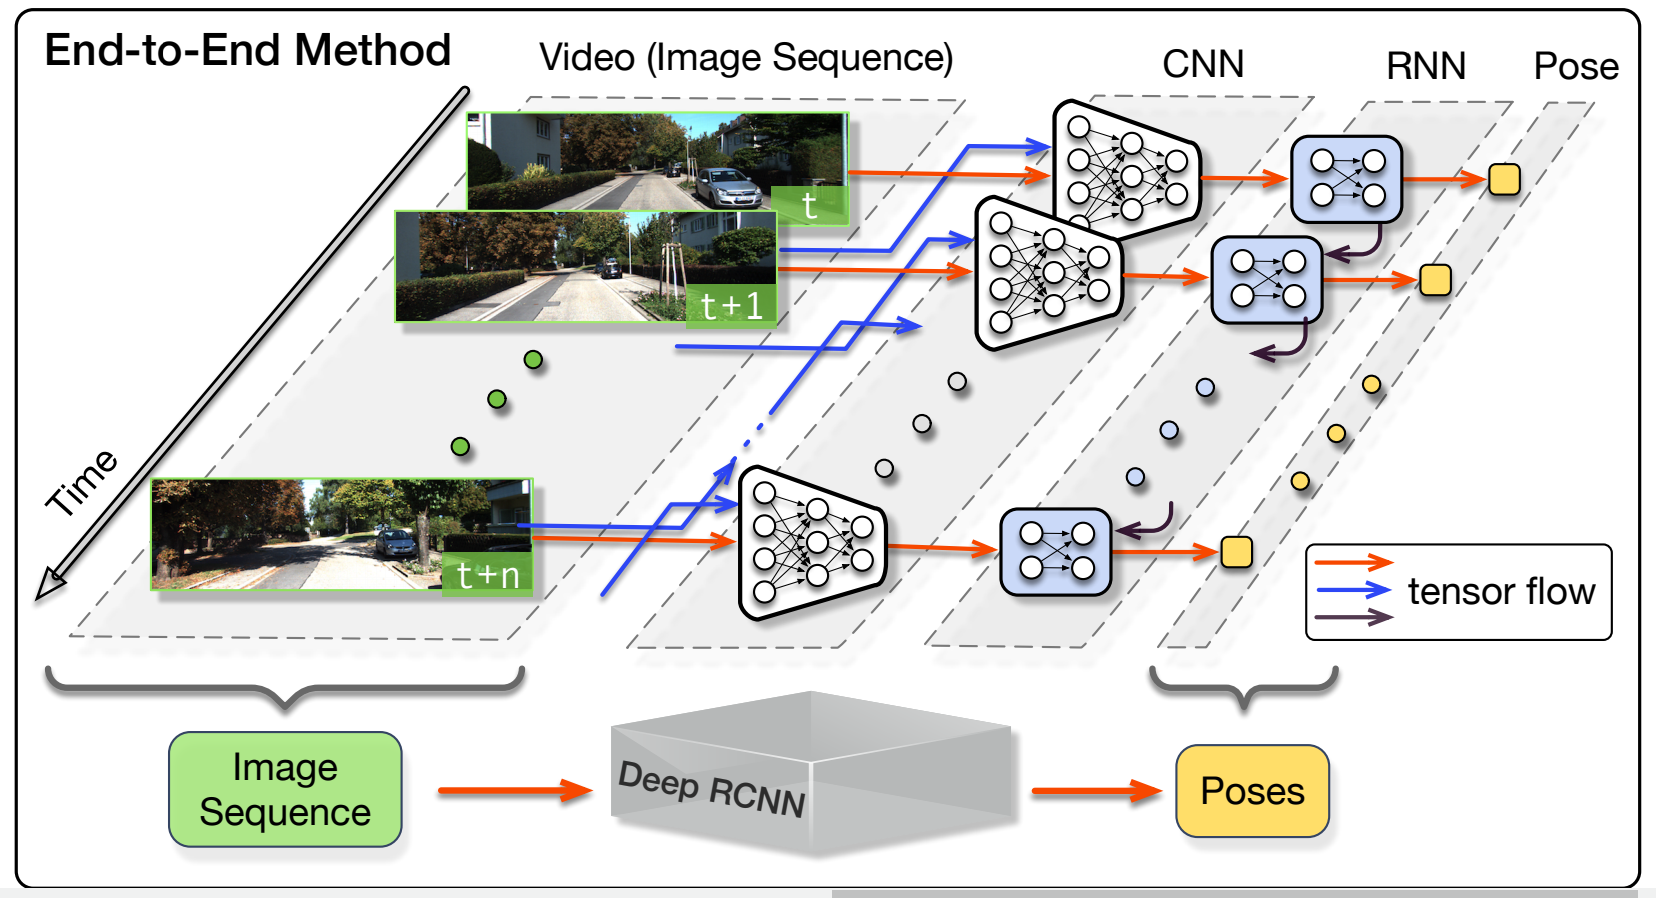
\includegraphics[width=0.9\linewidth]{images/deepvo.png}
		\caption{Motion estimation from image sequence}
	\end{figure}
		
	\cite{DEEPVO}
\end{frame}

\begin{frame}{More Applications}

	And much more:
	\begin{itemize}
		\item Video analysis
		\item Scene understanding
		\item Face recognition
		\item Pose tracking
		\item Crowd analysis
		\item Suspicious behaviour detection
		\item Data generation
		\item ...
	\end{itemize}
	
\end{frame}







